




Likewise, just as a tensor can be converted into a matrix, it can also be converted into a vector. This process is called vectorization:
\begin{definition}(Vectorization)\label{def:vectorization}
Let $\Tt\in\RR^{d_1\times d_2\times\cdots\times d_N}$. The \emph{vectorization} of $\Tt$ denoted as $\vectorize(\Tt)\in\RR^{d_1d_2\cdots d_N}$ is the vector obtained by concatenating its mode-$N$ fibers\footnote{Using the lexicographic order.}. For example, the vectorization of a tensor $\Tt\in\RR^{d_1\times d_2\times d_3}$ is given by:
$$\vectorize(\Tt) =    
[(\Tt_{1,1,:})\ \  (\Tt_{1,2,:})\ \  \cdots \ \ (\Tt_{d_1,d_2,:})]^\ts
=
\begin{tikzpicture}[baseline=\baseline]
    \tikzset{tensor/.style = {minimum size = 0.5cm,shape = circle,thick,draw=black,inner sep = 0pt}, edge/.style = {thick,line width=.4mm},every loop/.style={}}
    \def\y{0}
    \def\x{0}
    \node[tensor,fill=blue!10!white] (A) at (\x,\y){\scalebox{0.85}{$\Tt$}};
    \draw[edge] (\x+0.15,\y+0.2) -- (\x+0.5,\y+0.2) -- (\x+0.5,\y+0.1) -- (\x+1,\y+0.1) node [midway,above]
    {\scalebox{0.7}{\dimcolor{$d_1$}}};
     \draw[edge] (A) -- (\x+1,\y)node [right]
    {\scalebox{0.7}{\dimcolor{$d_2$}}};

    \draw[edge] (\x+0.15,\y-0.2) -- (\x+0.5,\y-0.2)-- (\x+0.5,\y-0.1)-- (\x+1,\y-0.1) node [midway,below]
    {\scalebox{0.7}{\dimcolor{$d_3$}}};
    \end{tikzpicture}\in\RR^{d_1d_2d_3}.
$$
\end{definition}

Vectorization is a flattening operation that converts a tensor of any order into a vector. Similarly to matricization, in tensor networks
the edge of the shape $
\begin{tikzpicture}[baseline=\baseline]
    \tikzset{tensor/.style = {minimum size = 0.5cm,shape = circle,thick,draw=black,inner sep = 0pt}, edge/.style = {thick,line width=.4mm},every loop/.style={}}
    \def\y{0}
    \def\x{0}
    \draw[edge] (\x+0.15,\y+0.2) -- (\x+0.5,\y+0.2) -- (\x+0.5,\y+0.1) -- (\x+1,\y+0.1) node [midway,above]
    {\scalebox{0.7}{\textcolor{gray}{$d_1$}}};
    \draw[edge] (\x+0.15,\y) -- (\x+1,\y)node [right]
    {\scalebox{0.7}{\textcolor{gray}{$d_2$}}};
    \draw[edge] (\x+0.15,\y-0.2) -- (\x+0.5,\y-0.2)-- (\x+0.5,\y-0.1)-- (\x+1,\y-0.1) 
node [midway,below]
    {\scalebox{0.7}{\dimcolor{$d_3$}}};
    \end{tikzpicture}
$ represents an edge of size $d_1d_2d_3$. In general, throughout this manuscript, convergent edges represent an edge whose size is the product of the sizes of all associated edges. Note that the vectorization of a tensor is equal to the vectorization\footnote{To be consistent with the definition of vectorization used in this book, the vectorization of a matrix is given by the concatenation of its rows, which is sometimes referred to as \emph{row-major vectorization}.Note that this is the default vectorizing operation, \textsf{ravel()}, of the \textsf{numpy} package in \textsf{Python}.} of the  mode-$1$ matricization of the tensor, i.e., for $\Tt\in\RR^{d_1\times d_2\cdots \times d_N}$, $\vectorize(\Tt) = \vectorize(\Tt_{(1)})$.




\subsection{Products}\label{sec:product}
Tensors can be combined or \textit{multiplied} using different types of operation. In this section, we provide graphical illustrations of different product operations.
\paragraph{Mode-$n$ Tensor Product}\label{par:mode-n-tensor-product}
The modes $n$ products, where a tensor is multiplied by a matrix along a specific mode, can be seen as a generalization of the matrix products. More precisely, the mode-$n$ product generalizes matrix-matrix multiplication along one particular mode. These include mode-$n$ products between tensors and matrices, as well as tensors and vectors.
\begin{enumerate}
\item \textbf{Mode-n product~(matrix).}\label{subsec:mode-n}
    The mode-$n$ product of a tensor $\Xt\in\RR^{d_1\times\cdots\times d_N}$ with a matrix $\Mb\in\RR^{m\times d_n}$ denoted as
    $\Xt\ttm n \Mb \in \RR^{d_1\times \cdots\times d_{n-1}\times m\times d_{n+1}\times\cdots\times d_N}$ is defined as the contraction of a tensor with a matrix along mode-$n$ of the tensor and mode-2 of the matrix~(column index), i.e., 
    $$
  \Xt\ttm n \Mb
=
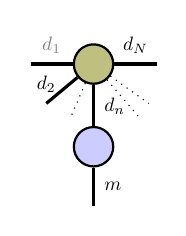
\begin{tikzpicture}[baseline=-0.5ex]
    \tikzset{tensor/.style = {minimum size = 0.5cm,shape = circle,thick,draw=black,inner sep = 0pt}, edge/.style = {thick,line width=.4mm},every loop/.style={}}
    \def\x{6}
    \node[tensor,fill=blue!20!white] (M) at (\x,-1.05) {$\Mb$};
    \node[tensor,fill=green!50!red!50!white] (At) at (\x,0) {$\Xt$};
    \draw[edge] (At) -- (\x-0.8,0) node [midway,above] {\scalebox{0.7}{\textcolor{gray}{$d_1$}}};
    \draw[edge] (At)-- (\x-0.6,-0.5) node [above]{\scalebox{0.7}{\dimcolor{$d_2$}}};
    \draw[edge] (At) -- (\x+0.8,0) node [midway,above] {\scalebox{0.7}{\dimcolor{$d_N$}}};;
    \draw[dotted] (At) -- (\x-0.3,-0.7);
    \draw[edge] (At) -- (\x,-0.8) node [midway,right] {\scalebox{0.7}{\dimcolor{$d_n$}}};
    \draw[dotted] (At) -- (\x+0.6,-0.7);
    \draw[dotted] (At) -- (\x+0.7,-0.5);
    \draw[edge] (M) -- (\x,-1.8) node [midway,right] {\scalebox{0.7}{\dimcolor{$m$}}};;
    \end{tikzpicture}
\in\RR^{d_1\times  \dots\times d_{n-1}\times m \times d_{n+1}\times \dots\times d_N}.
$$
The operation contracts the tensor's $n$-th mode with the matrix's second mode~(column), replacing the original dimension $d_n$ with a new dimension $m$. For $\Ab\in\RR^{d_n\times n},\Bb\in\RR^{d_m\times m}$ and $\Xt\in\RR^{d_1\times\cdots\times d_N}$ with distinct modes $n\neq m$, the order of multiplication does not matter, i.e.,
$$
\Xt\ttm n \Ab \ttm m \Bb = 
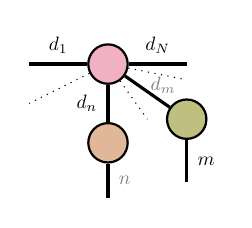
\begin{tikzpicture}[baseline=-0.5ex]
    \tikzset{tensor/.style = {minimum size = 0.5cm,shape = circle,thick,draw=black,inner sep = 0pt}, edge/.style = {thick,line width=.4mm},every loop/.style={}}
    \def\x{0}
    \def\y{0}
    \node[tensor,fill=blue!20!red!30!white] (Xt) at (\x,\y) {$\Xt$};
    \node[tensor,fill=green!30!red!40!white] (A) at (\x,\y-1) {$\Ab$};
    \node[tensor,fill=green!50!red!50!white] (B) at (\x+1,\y-0.7) {$\Bb$};
    \draw[edge] (Xt) -- (\x-1,\y) node [midway,above] {\scalebox{0.7}{\dimcolor{$d_1$}}};
    \draw[dotted] (Xt) -- (\x-1,\y-0.5);
    \draw[edge] (Xt) -- (\x+1,\y) node [midway,above] {\scalebox{0.7}{\dimcolor{$d_N$}}};
    \node[draw=none] () at (\x+0.7,\y-0.27) {\scalebox{0.7}{\textcolor{gray}{$d_m$}}};
    \draw[edge] (Xt) -- (A) node [midway,left] {\scalebox{0.7}{\dimcolor{$d_n$}}};
    \draw[edge] (A) -- (\x,\y-1.7) node [midway,right] {\scalebox{0.7}{\textcolor{gray}{$n$}}};
    \draw[edge] (Xt) -- (B);
    \draw[edge] (B) -- (\x+1,\y-1.5) node [midway,right] {\scalebox{0.7}{\dimcolor{$m$}}};
    \draw[dotted] (Xt) -- (\x+1,\y-0.2);
    \draw[dotted] (Xt) -- (\x+0.5,\y-0.7);
    \end{tikzpicture}
= \Xt\ttm m\Bb\ttm n \Ab,~~\text{For}~~n\neq m.
$$
However, if $m = n$ the order of the products is important. In particular, if $\Ab\in\RR^{n\times d_n}$ and $\Bb\in\RR^{p\times n}$ we have $(\Xt\ttm n \Ab) \ttm n \Bb = \Xt\ttm n(\Bb\Ab)$, whereas the product $(\Xt\ttm n \Bb) \ttm n \Ab$ is not valid unless $n=d_n=p$.
The mode-$n$ tensor product can be seen as a generalization of classical matrix multiplication. In particular,
we can recover matrix products with mode-$1$ and mode-$2$ products of an order 2 tensor: 
if $\Ab\in\RR^{m\times n}$, $\Bb\in\RR^{p\times n}$ and $\Cb\in\RR^{d\times m}$, then
\begin{align*}
\Ab\ttm2 \Bb
=
\begin{tikzpicture}[baseline=\baseline]
   \tikzset{tensor/.style = {minimum size = 0.5cm,shape = circle,thick,draw=black,inner sep = 0pt}, edge/.style = {thick,line width=.4mm},every loop/.style={}}
    \def\y{0}
    \def\x{0}
    \node[tensor,fill=red!50!white] (A) at (\x,\y){\scalebox{0.85}{$\Ab$}};
    \node[tensor,fill=blue!50!white] (B) at (\x+1,\y){\scalebox{0.85}{$\Bb$}};
    \draw[edge] (A) -- (B) node [above,midway] {\scalebox{0.7}{\dimcolor{$n$}}};
    \draw[edge] (\x-0.25,\y) -- (\x-0.6,\y)  node [midway,above] {\scalebox{0.7}{\dimcolor{$m$}}};
    \draw[edge] (\x+1.25,\y) -- (\x+1.6,\y)  node [midway,above] {\scalebox{0.7}{\dimcolor{$p$}}};
    \end{tikzpicture}
    = \Ab\Bb^\ts\in\RR^{m\times p},
\end{align*}
\begin{align*}
    \Ab\ttm1 \Cb =
    \begin{tikzpicture}[baseline=\baseline]
   \tikzset{tensor/.style = {minimum size = 0.5cm,shape = circle,thick,draw=black,inner sep = 0pt}, edge/.style = {thick,line width=.4mm},every loop/.style={}}
    \def\y{0}
    \def\x{0}
    \node[tensor,fill=red!20!white] (C) at (\x,\y){\scalebox{0.85}{$\Cb$}};
    \node[tensor,fill=red!50!white] (A) at (\x+1,\y){\scalebox{0.85}{$\Ab$}};
    \draw[edge] (C) -- (A) node [above,midway] {\scalebox{0.7}{\dimcolor{$m$}}};
    \draw[edge] (\x-0.25,\y) -- (\x-0.6,\y)  node [midway,above] {\scalebox{0.7}{\dimcolor{$d$}}};
    \draw[edge] (\x+1.25,\y) -- (\x+1.6,\y)  node [midway,above] {\scalebox{0.7}{\dimcolor{$n$}}};
    \end{tikzpicture}
    = \Cb\Ab\in\RR^{d\times n}.
\end{align*}

